\documentclass[12pt, a4paper]{article}
\usepackage[utf8]{inputenc}
\usepackage{listings}
\usepackage{courier}
\usepackage{fancyhdr}
\usepackage{color}
\usepackage{xcolor}
\usepackage{caption}
\usepackage{graphicx}


\definecolor{light-gray}{gray}{0.95}

\lstset{
 showspaces=false,
 showtabs=false,
 frame=none,
 tabsize=2,
 breaklines=true,
 numbers=none,
 showstringspaces=false,
 breakatwhitespace=true,
 escapeinside={(*@}{@*)},
 keywordstyle=\bfseries,
 basicstyle=\footnotesize\ttfamily,
}

\newcommand{\code}[1]{{\footnotesize\texttt{#1}}}

\setlength\parindent{0pt} % Indentazione paragrafi
\setlength{\parskip}{1ex plus 0.5ex minus 0.2ex} % Spaziatura paragrafi

\title{SDN controller clustering \\ \large Computer Networks module - SDN assignment}
\author{Michele Zanotti}
\date{Spring term 2018}

\pagestyle{fancy}
\fancyhf{}
\lhead{Computer Networks}
\rhead{SDN assignment}
\rfoot{\thepage}

\begin{document}

\maketitle


\section*{Overview}
In this paper are proposed four different lab activities meant to teach how to implement
a cluster of controllers inside Mininet using some of the most common available methods.
Each activity focuses on a single method and uses as reference the topology
diagram showed in figure \ref{fig:topology-1}.

In particular, in each activity the following methods will be explained:
\begin{itemize}
  \item \textbf{Activity 1}: implement a network with multiple local controllers using a python
  script and the middle-level Mininet API
  \item \textbf{Activity 2}: implement a network with multiple remote controllers using a python
  script and the middle-level Mininet API
  \item \textbf{Activity 3}: implement a network with multiple local controllers using a python
  script and the high-level Mininet API
  \item \textbf{Activity 4}: build a cluster of controllers using the tool
  \emph{miniedit} provided by Mininet
\end{itemize}

The paper also includes a fifth lab activity, which is a challange meant
to let the reader test the knowledge acquired with the execution of the previous
four activities.

\begin{figure}[htb]
	\centering
	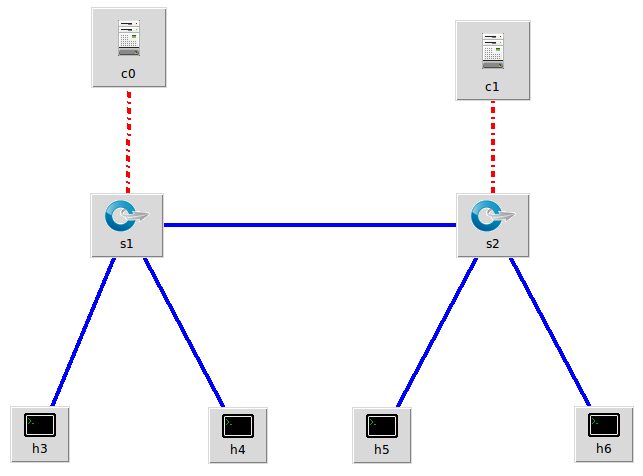
\includegraphics[width=0.9\linewidth]{img/topology-1.png}
	\caption{the simple topology that will be used as reference in the first four
  activities. The topology includes two switches, each one connected to a different
  controller. The two controllers \emph{c0} and \emph{c1} can be assumed local or
  remote depending on the lab activity.}
	\label{fig:topology-1}
\end{figure}


\section*{Lab activity 1}





\subsection*{Learning objectives}
After finishing this lab activity you will be able to:
\begin{itemize}
  \item Implement a cluster of local controller inside Mininet using the python
  middle-level Mininet API
  \item Test the network connectivity and the performance of a network which
  includes a cluster of local controllers
  \item Understand the main functions provided by the middle-level Mininet API required
  to implement a cluster of local controllers
\end{itemize}






\subsection*{Scenario}
In this activity you will implement the simple topology shown in figure *** using
a Python script and the middle-level API provided by Mininet. The two controllers
showned in the topology diagram will be local controllers for this activity.
The topology has two different switches: each one will be connected to a different
local controller.

Begin by creating a new Python script, then import Mininet classes required for
this activity and define the function that will be used to create the topology.
Inside the body of this function, create a new Mininet netowrk and add to it the
required hosts, switches, links and controllers. After writing the script, execute
it to create the network and test its connectivity and performance.

This lab activity assumes you are proficient in [...]. A basic knowledge of the
Python programming language is also assumed.





\subsection*{Task 1: write the skeleton of the Python script}
\subsubsection*{Step 1}
Create a new python script and edit with the text editor you prefer. If your editing
it inside the Mininet virtual machine, it is suggested to use Vim text editor.

\subsubsection*{Step 2}
Import the Python classes from the Mininet API:
\begin{lstlisting}
#!/usr/bin/python
from mininet.net import Mininet
from mininet.node import Controller, OVSSwitch
from mininet.cli import CLI
from mininet.log import setLogLevel, info
\end{lstlisting}

\subsubsection*{Step 3}
Make the script executable onyl as a program, set the log level to ``info''
and call the function \code{multiControllerNet()}, which will be defined in the next
step:
\begin{lstlisting}
if __name__ == '__main__':
    setLogLevel( 'info' )
    multiControllerNet()
\end{lstlisting}

\subsubsection*{Step 4}
Define the function that will be used to create the topology:
\begin{lstlisting}
def multiControllerNet():
\end{lstlisting}

\subsubsection*{Step 6}
Inside the body of the function \code{multiControllerNet()} create a new Mininet
network:
\begin{lstlisting}
net = Mininet( controller=Controller, switch=OVSSwitch )
\end{lstlisting}

The Mininet network is created invoking the Mininet constructor: the parameters
passed to the constructor are the Controller class and the OVSSwitch class, therefore
the Stanford/OpenFlow reference controllers and Open vSwitch switches will be used
in the network we are goind to create. Note that these two classes are
the default parameters in the Mininet constructor, so it is not really necessary
to specify them.

\subsubsection*{Step 7}
Save the text file as ``\emph{controllers-1.py}'' in your custom directory inside
the mininet virtual machine.





\subsection*{Task 2: add hosts to the network}
\subsubsection*{Step 1}
Inside the body of the function \code{multiControllerNet()} add the following line
of code in order to print to the console that hosts are being created:
\begin{lstlisting}
info( "*** Creating hosts \n" )
\end{lstlisting}

\subsubsection*{Step 2}
Still inside the body of the function \code{multiControllerNet()}, create the
four hosts required for the topology by adding them to the mininet network
previously created:
\begin{lstlisting}
h1 = net.addHost('h3')
h2 = net.addHost('h4')
h3 = net.addHost('h5')
h4 = net.addHost('h6')
\end{lstlisting}
The function used to add the hosts to the network is \code{addHost('name')}, which
accept as parameter the name of the host that will be created. The hosts names in
this network therefore will we \code{h3}, \code{h4}, \code{h5} and \code{h6}.





\subsection*{Task 3: add switches to the network}
\subsubsection*{Step 1}
Inside the body of the function \code{multiControllerNet()} add the following line
of code in order to print to the console that switches are being created:
\begin{lstlisting}
info( "*** Creating switches \n" )
\end{lstlisting}

\subsubsection*{Step 2}
Still inside the body of the function \code{multiControllerNet()}, create the
two switches required for the topology by adding them to the mininet network
previously created:
\begin{lstlisting}
s1 = net.addSwitch('s1')
s2 = net.addSwitch('s2')
\end{lstlisting}







\subsection*{Task 4: create links between nodes}
\subsubsection*{Step 1}
Inside the body of the function \code{multiControllerNet()} add the following line
of code in order to print to the console that links are being created:
\begin{lstlisting}
info( "*** Creating links \n" )
\end{lstlisting}

\subsubsection*{Step 2}
Still inside the body of the function \code{multiControllerNet()}, create four
links between the hosts and the switches and the link between the two switches:
\begin{lstlisting}
net.addLink( h3, s1 )
net.addLink( h4, s1 )
net.addLink( h5, s2 )
net.addLink( h6, s2 )
net.addLink( s1, s2 )
\end{lstlisting}








\subsection*{Step 5: create controllers} \label{sec:step-5}
In this step we are going to create two local SDN controllers. The code we have to
add to the script is the following:

\code{info( "*** Creating (reference) controllers\textbackslash n" )} \\
\code{c1 = net.addController( 'c1', port=6633 )} \\
\code{c2 = net.addController( 'c2', port=6634 )}

Note that we specified a different TCP port for each controller (the controllers
will listen on the specified port for switches that want to set up a connection).

\textbf{Why did we specify a different port for each controller?}

\hrulefill

\hrulefill
% Because each swtich has to setup one TCP connection to each controller and
% it's not possible having more than one TCP connection on the same port, so
% specifying two different ports makes it possible to connect one single switch
% to multiple controllers.


\subsection*{Step 6: start the network}
After adding all the required nodes to the network we can finally start it. In order
to do that, we have to build the mininet network and start the controllers and the
switches:

\code{info( "*** Starting network\textbackslash n" )} \\
\code{net.build()} \\
\code{c1.start()} \\
\code{c2.start()} \\
\code{s1.start( [ c1 ] )} \\
\code{s2.start( [ c2 ] )}

In the last two lines of code we used the function start() to start the two switches,
passing as parameter

After this step, the python script required to build the topology for the task one
is completed. The full script is shown in listing \ref{lst:task-1-complete-script}.



\subsection{Step 7: test network connectivity and performance}
The final step is execute the script and test the created topology: try to verify
the network connectivity between all hosts and the bandwidth between \code{h3} and \code{h6}.
Write in the lines below the commands you used and the results you obtained.

\hrulefill

\hrulefill

\hrulefill

\begin{lstlisting}[label=lst:task-1-complete-script, caption=Task 1 complete python script]
#!/usr/bin/python
from mininet.net import Mininet
from mininet.node import Controller, OVSSwitch
from mininet.cli import CLI
from mininet.log import setLogLevel, info

def multiControllerNet():
    net = Mininet( controller=Controller, switch=OVSSwitch )

    info( "*** Creating hosts\n" )
    h1 = net.addHost('h3')
    h2 = net.addHost('h4')
    h3 = net.addHost('h5')
    h4 = net.addHost('h6')

    info( "*** Creating switches\n" )
    s1 = net.addSwitch( 's1' )
    s2 = net.addSwitch( 's2' )

    info( "*** Creating links\n" )
    net.addLink( h3, s1 )
    net.addLink( h4, s1 )
    net.addLink( h5, s2 )
    net.addLink( h6, s2 )
    net.addLink( s1, s2 )

    info( "*** Creating (reference) controllers\n" )
    c1 = net.addController( 'c1', port=6633 )
    c2 = net.addController( 'c2', port=6634 )

    info( "*** Starting network\n" )
    net.build()
    c1.start()
    c2.start()
    s1.start( [ c1 ] )
    s2.start( [ c2 ] )

    info( "*** Running CLI\n" )
    CLI( net )

    info( "*** Stopping network\n" )
    net.stop()

if __name__ == '__main__':
    setLogLevel( 'info' )  # for CLI output
    multiControllerNet()
\end{lstlisting}

\lstset{
 upquote=true,
 showspaces=false,
 showtabs=false,
 frame=none,
 tabsize=2,
 breaklines=true,
 numbers=none,
 showstringspaces=false,
 breakatwhitespace=true,
 escapeinside={(*@}{@*)},
 keywordstyle=\bfseries,
 basicstyle=\footnotesize\ttfamily,
}

\section*{Lab activity 2}

\subsection*{Topology diagram}
\begin{figure}[htb]
	\centering
	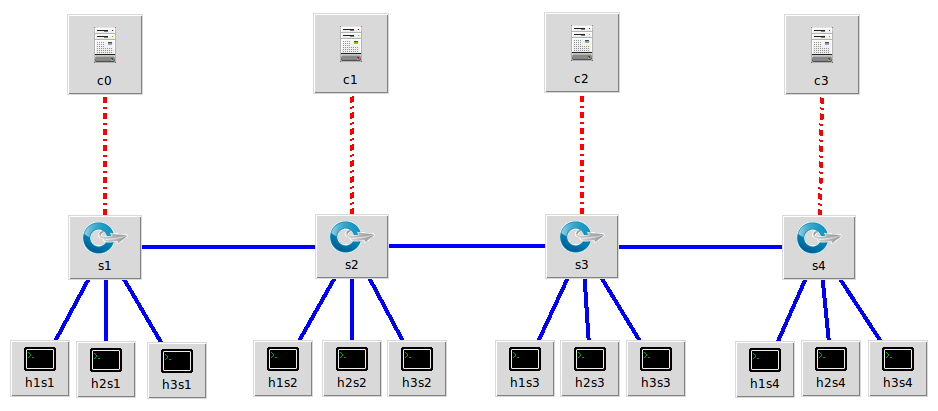
\includegraphics[width=1\linewidth]{img/topology-2.png}
	\caption{the topology that will be implemented during this lab activity.
  It is a linear topology with four switches connected to each other,
  each one connected to three hosts. Each switch is linked to a different
  SDN controller. All the controllers can be assumed local.}
	\label{fig:topology-2}
\end{figure}

\subsection*{Learning objectives}
After finishing this lab activity you will be able to:
\begin{itemize}
  \item create a custom switch class that extends the OVSSwitch class provided
  by the Mininet Python API
  \item implement a cluster of local/remote controllers inside Mininet using a custom
  switch class and the topology classes provided by the Mininet high-level API
  \item implement more complex topologies with multiple controllers using a
  few lines of Python code
  \item reflect upon the method used in this activity for implementing a cluster of controllers
  and compare it with the method shown in Activity 1, focusing on the advantages
  and disadvantages of each method
  \item test the network connectivity and the performance of a network with multiple
  controllers.
\end{itemize}






\subsection*{Scenario}
In this activity you will implement the topology shown in figure \ref{fig:topology-2} using
a Python script and the classes provided by the high-level Mininet API, which
represent topology templates. In order to use these classes for creating a network
with multiple controllers, you will have to define a new switch class that extends
the standard OVSSwitch class provided by the API.

Begin by creating a new Python script and importing the required Mininet classes.
Create the controllers shown in the topology diagram and define
a custom switch class which extends the class \code{OVSSwitch}. Define a function for creating
the network and inside its body use one of the topology templates provided
by the API to implement the required topology.
After writing the script, execute it and test the network connectivity and its
performance. To conclude, answer the questions proposed in the last task.

This lab activity assumes that:
\begin{itemize}
  \item you are proficient in SDN networks
  \item you are proficient in Mininet network emulator
  \item you have a basic knowledge of Python object-oriented
  \item you have already completed Activity 1.
\end{itemize}

The activity is inspired by the script \textit{controllers.py} \parencite{ref-6} included in the
examples provided by Mininet, which can therefore be used as
an additional example of how a topology with multiple controllers can be implemented
inside Mininet using a Python script and defining a custom switch class.





\subsection*{Task 1: create the controllers}
\subsubsection*{Step 1}
Create a new Python script and edit it with the text editor you prefer. If you're editing
it inside the Mininet virtual machine, it is suggested to use Vim text editor.

\subsubsection*{Step 2}
Import the required Python classes from the Mininet API:
\begin{lstlisting}
#!/usr/bin/Python
from mininet.net import Mininet
from mininet.node import OVSSwitch, Controller
from mininet.topo import LinearTopo
from mininet.log import setLogLevel
from mininet.cli import CLI
\end{lstlisting}

\subsubsection*{Step 3}
Create the four required controllers, specifying for each one a different name and
a different TCP port:
\begin{lstlisting}
c0 = Controller( 'c0', port=6633 )
c1 = Controller( 'c1', port=6634 )
c2 = Controller( 'c2', port=6635 )
c3 = Controller( 'c3', port=6636 )
\end{lstlisting}

\subsubsection*{Step 4}
Create a new array and initialize it with the four created controllers:
\begin{lstlisting}
controllers = [c0, c1, c2, c3]
\end{lstlisting}
This array will be used later in the script to easily add all the controllers
to the network using a for loop (see Step 4 of Task 3).

\subsubsection*{Step 5}
Create a map that associates each switch to the relative controller:
\begin{lstlisting}
cmap = { 's1': c0, 's2': c1, 's3': c2, 's4' : c3 }
\end{lstlisting}






\subsection*{Task 2: create a custom switch class}
\subsubsection*{Step 1}
Define a new class called \code{MultiSwitch} wich extends the class
\code{OVSSwitch} provided by the Mininet API:
\begin{lstlisting}
class MultiSwitch( OVSSwitch ):
\end{lstlisting}

\subsubsection*{Step 2}
Overwrite the method \code{start} of the superclass \code{OVSSwitch}:
\begin{lstlisting}
def start( self, controllers ):
  return OVSSwitch.start( self, [ cmap[ self.name ] ] )
\end{lstlisting}
The method simply returns the result of the call to the method \code{start} of the
superclass passing as parameter the controller associated to the switch name, as defined by
the map \code{cmap} previously created. In this way each switch will connect to
the relative controller according to the map \code{cmap}.






\subsection*{Task 3: define a function that creates the topology}
\subsubsection*{Step 1}
Define a new function called ``multiControllerNet'':
\begin{lstlisting}
def multiControllerNet():
\end{lstlisting}

\subsubsection*{Step 2}
Create a new linear topology using the class \code{LinearTopo} provided by
the API, specifying as parameters the number of switches \code{k} and the
number of hosts per switch \code{n}:
\begin{lstlisting}
topo = LinearTopo( k=4, n=3 )
\end{lstlisting}

\subsubsection*{Step 3}
Create a new Mininet network, specifying as constructor parameters the topology
called \code{topo} created in the previous step, the class \code{MultiSwitch}
defined in task 2 and the value \code{build=False} for preventing Minined to build
the network immediately:
\begin{lstlisting}
net = Mininet( topo=topo, switch=MultiSwitch, build=False)
\end{lstlisting}

\subsubsection*{Step 4}
Add the controllers to the network:
\begin{lstlisting}
for c in controllers:
  net.addController(c)
\end{lstlisting}

\subsubsection*{Step 5}
Build the network and start it:
\begin{lstlisting}
net.build()
net.start()
\end{lstlisting}

\subsubsection*{Step 6}
Start the CLI and stop the network:
\begin{lstlisting}
CLI( net )
net.stop()
\end{lstlisting}




\subsection*{Task 4: finalize the script and save it}
\subsubsection*{Step 1}
Make the script executable only as a program and set the CLI verbosity level
to ``info'':
\begin{lstlisting}
if __name__ == '__main__':
    setLogLevel( 'info' )
    multiControllerNet()
\end{lstlisting}

\subsubsection*{Step 2}
Save the text file as ``\emph{activity-2.py}'' in your custom directory inside
the mininet virtual machine.






\subsection*{Task 5: execute the script and test the network}
After finishing the task 4 the script for implementing the required topology is
completed. The full script is shown in listing \ref{lst:activity-2-script} at the
bottom of this activity.

\subsubsection*{Step 1}
Execute the script as root: \\
\code{\$ sudo python activity-2.py}

\subsubsection*{Step 2}
Test the created topology: verify the network connectivity between all hosts.
Write in the lines below the commands you used and the results you obtained.

\hrulefill

\hrulefill

\hrulefill

\hrulefill

\subsubsection*{Step 3}
Verify the bandwidth and the delay between the hosts \code{h1s1} and \code{h3s4}.
Write in the lines below the commands you used and the results you obtained.

\hrulefill

\hrulefill

\hrulefill

\hrulefill





\subsection*{Task 6: reflection}
\subsubsection*{1 - In this activity you implemented a network with multiple
controllers using a custom switch class and the high-level API. Which are
the advantages of using this method insted of the one used in Activity 1? What
about the disadvantages?}
\hrulefill

\hrulefill

\hrulefill

\hrulefill


\subsubsection*{2 - In this activity the topology shown in figure \ref{fig:topology-2}
was implemented assuming that all the controllers were local controllers. How would
you have to change the Python script you created in this activity in order
to use remote controllers instead of local ones?}
\hrulefill

\hrulefill

\hrulefill

\hrulefill


\subsubsection*{3 - Try to modify the script you realized in order to have only
two controllers instead of four, each one linked to two different switches. Each
switch must be linked to a controller. }
\hrulefill

\hrulefill

\hrulefill

\hrulefill






\lstset{
 upquote=true,
 showspaces=false,
 showtabs=false,
 frame=single,
 tabsize=2,
 breaklines=true,
 numbers=left,
 showstringspaces=false,
 breakatwhitespace=true,
 escapeinside={(*@}{@*)},
 keywordstyle=\bfseries,
 basicstyle=\scriptsize\ttfamily,
}

\begin{minipage}{\linewidth}
\begin{lstlisting}[label=lst:activity-2-script, caption=the complete Python script required for Activity 2]
#!/usr/bin/Python
from mininet.net import Mininet
from mininet.node import OVSSwitch, Controller
from mininet.topo import LinearTopo
from mininet.log import setLogLevel
from mininet.cli import CLI

c0 = Controller( 'c0', port=6633 )
c1 = Controller( 'c1', port=6634 )
c2 = Controller( 'c2', port=6635 )
c3 = Controller( 'c3', port=6636 )

controllers = [c0, c1, c2, c3]
cmap = { 's1': c0, 's2': c1, 's3': c2, 's4' : c3 }


class MultiSwitch( OVSSwitch ):
  def start( self, controllers ):
    return OVSSwitch.start( self, [ cmap[ self.name ] ] )


def multiControllerNet():
  topo = LinearTopo( k=4, n=3 )
  net = Mininet( topo=topo, switch=MultiSwitch, build=False)

  for c in controllers:
    net.addController(c)

  net.build()
  net.start()
  CLI( net )
  net.stop()

if __name__ == '__main__':
  setLogLevel( 'info' )
  multiControllerNet()
\end{lstlisting}
\end{minipage}


\end{document}
